\documentclass[10pt, letterpaper]{article}
\usepackage[utf8]{inputenc}
\usepackage{amsmath}
\usepackage{amssymb}
\usepackage{bbm}
\usepackage{booktabs}
\usepackage{caption}
\usepackage{color}
\usepackage[shortlabels]{enumitem}
\usepackage{fancyhdr}
\usepackage{hyperref}
\usepackage{geometry}
\geometry{a4paper,scale=0.8}
\usepackage{graphicx}
\graphicspath{ {./img/}}
\usepackage{listings}
\usepackage{mathtools}
\usepackage{mathrsfs}
\usepackage{setspace}
\renewcommand{\baselinestretch}{1.3}

% set-up header & footer
\pagestyle{empty}
\fancyhf{}
\cfoot{\thepage}
\lhead{%
\textbf{University of California, Berkeley} \\
Department of Civil \& Environ. Eng.
}
\rhead{\textbf{CS 285 Deep Reinforcement Learning}\\\date{\today}}

\title{%
    \textbf{Homework 2}
}
\author{Juanwu Lu (3037432593)\\ \small(M.Sc. Civil Engineering, UC Berkeley)}
\date{}

% set-up code listing
\definecolor{dkgreen}{rgb}{0,0.6,0}
\definecolor{gray}{rgb}{0.5,0.5,0.5}
\definecolor{manuve}{rgb}{0.58,0,0.82}

\lstset{frame=tb,
    language=Python,
    aboveskip=3mm,
    belowskip=3mm,
    showstringspaces=false,
    columns=flexible,
    basicstyle={\small\ttfamily},
    numbers=none,
    numberstyle=\tiny\color{gray},
    keywordstyle=\color{blue},
    commentstyle=\color{dkgreen},
    stringstyle=\color{manuve},
    breaklines=true,
    breakatwhitespace=true,
    tabsize=3
}

\begin{document}
    \maketitle
    \captionsetup[figure]{labelfont={bf},labelformat={default},labelsep=period,name={Figure}}
    \captionsetup[table]{labelfont={bf},labelformat={default},labelsep=period,name={TABLE}}
    \thispagestyle{fancy}
    \pagestyle{plain}

    % Experiment 1
    \section*{Experiment 1 CartPole}
    \textbf{Answers:}
    \begin{itemize}
        \item The \textbf{reward-to-go} estimator has a better performance without advantage-standardization. Compare the green with orange curves in both figure 1(a) and (b), reward-to-go value estimators converge faster and are more stable across the training process.
        \item From my experiment results, advantage standardization helps in small batch experiments, but does not in large batch experiments.
        \item From my experiment results, batch size did make an impact to the training, with a larger batch size helps stablize the training.
    \end{itemize}

    \begin{figure}[thbp]
        \centering
        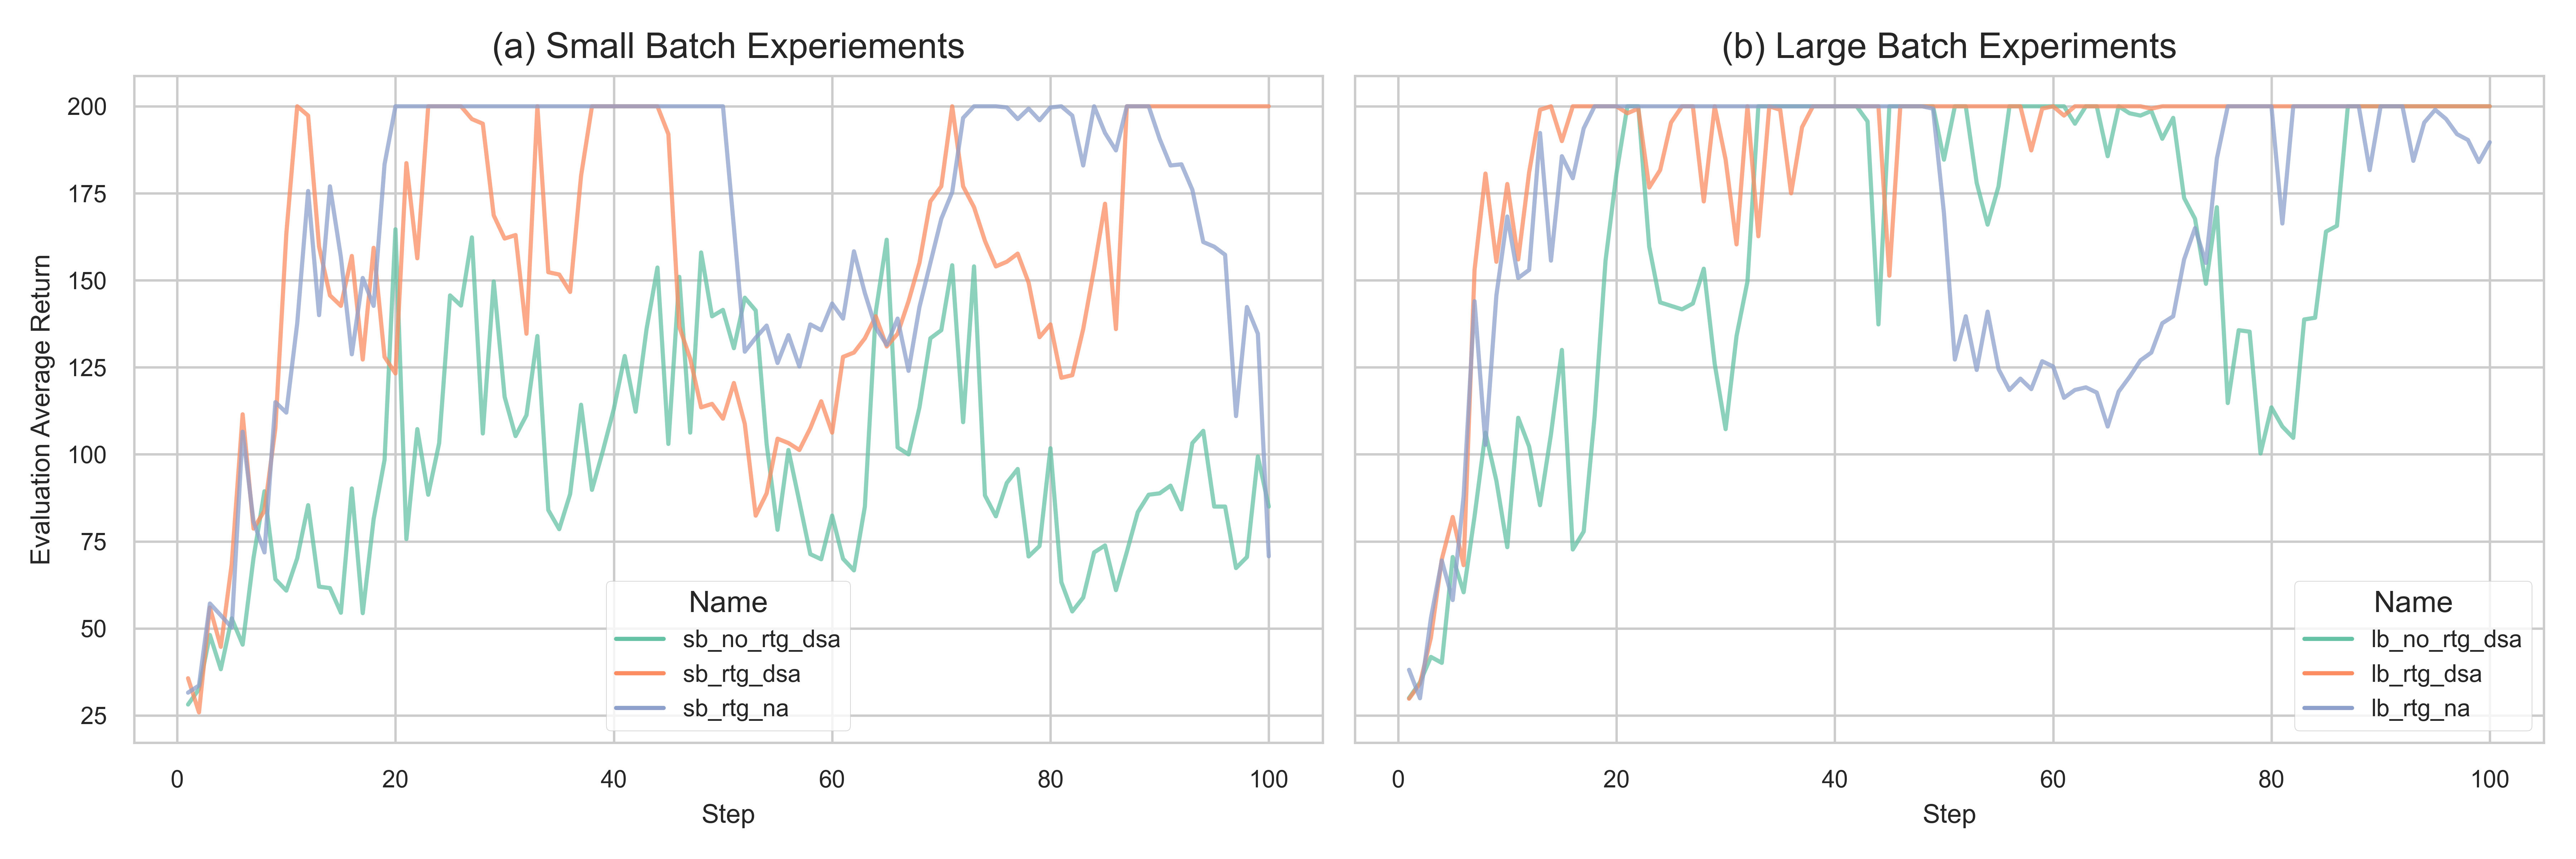
\includegraphics[width=\textwidth]{exp_01.png}
        \caption{Visualization of learning curves for (a) small batch experiments and (b) large batch experiments.}
        \label{fig:1}
    \end{figure}

    \textbf{Command-line Codes}
    \begin{lstlisting}
        echo 'Running small batch w/o reward_to_go w/ standardized_advatages';
        python $1 --env_name CartPole-v0 -n 100 -b 1000 -dsa --exp_name q1_sb_no_rtg_dsa;

        echo 'Running small batch w/ reward_to_go w/ standardized_advatages'; 
        python $1 --env_name CartPole-v0 -n 100 -b 1000 -rtg -dsa --exp_name q1_sb_rtg_dsa;

        echo 'Running small batch w/ reward_to_go w/o standardized_advatages';
        python $1 --env_name CartPole-v0 -n 100 -b 1000 -rtg --exp_name q1_sb_rtg_na;

        echo 'Running large batch w/o reward_to_go w/ standardized_advatages';
        python $1 --env_name CartPole-v0 -n 100 -b 5000 -dsa --exp_name q1_lb_no_rtg_dsa;

        echo 'Running large batch w/ reward_to_go w/ standardized_advatages'; 
        python $1 --env_name CartPole-v0 -n 100 -b 5000 -rtg -dsa --exp_name q1_lb_rtg_dsa;

        echo 'Running large batch w/ reward_to_go w/o standardized_advatages';
        python $1 --env_name CartPole-v0 -n 100 -b 5000 -rtg --exp_name q1_lb_rtg_na;
    \end{lstlisting}

    \section*{Experiment 2 InvertedPendulum}

    \textbf{Answers:}
    
    From my experiments, the optimal setting combination is \texttt{b*=500} and \texttt{r*=0.01}. Using this setting, I obtain a learning curve as shown in figure 2. Although this settings reaches a best score 1000 the fastest, the average return is unstable and shows occasion extreme decays.
    
    \begin{figure}[thbp]
        \centering
        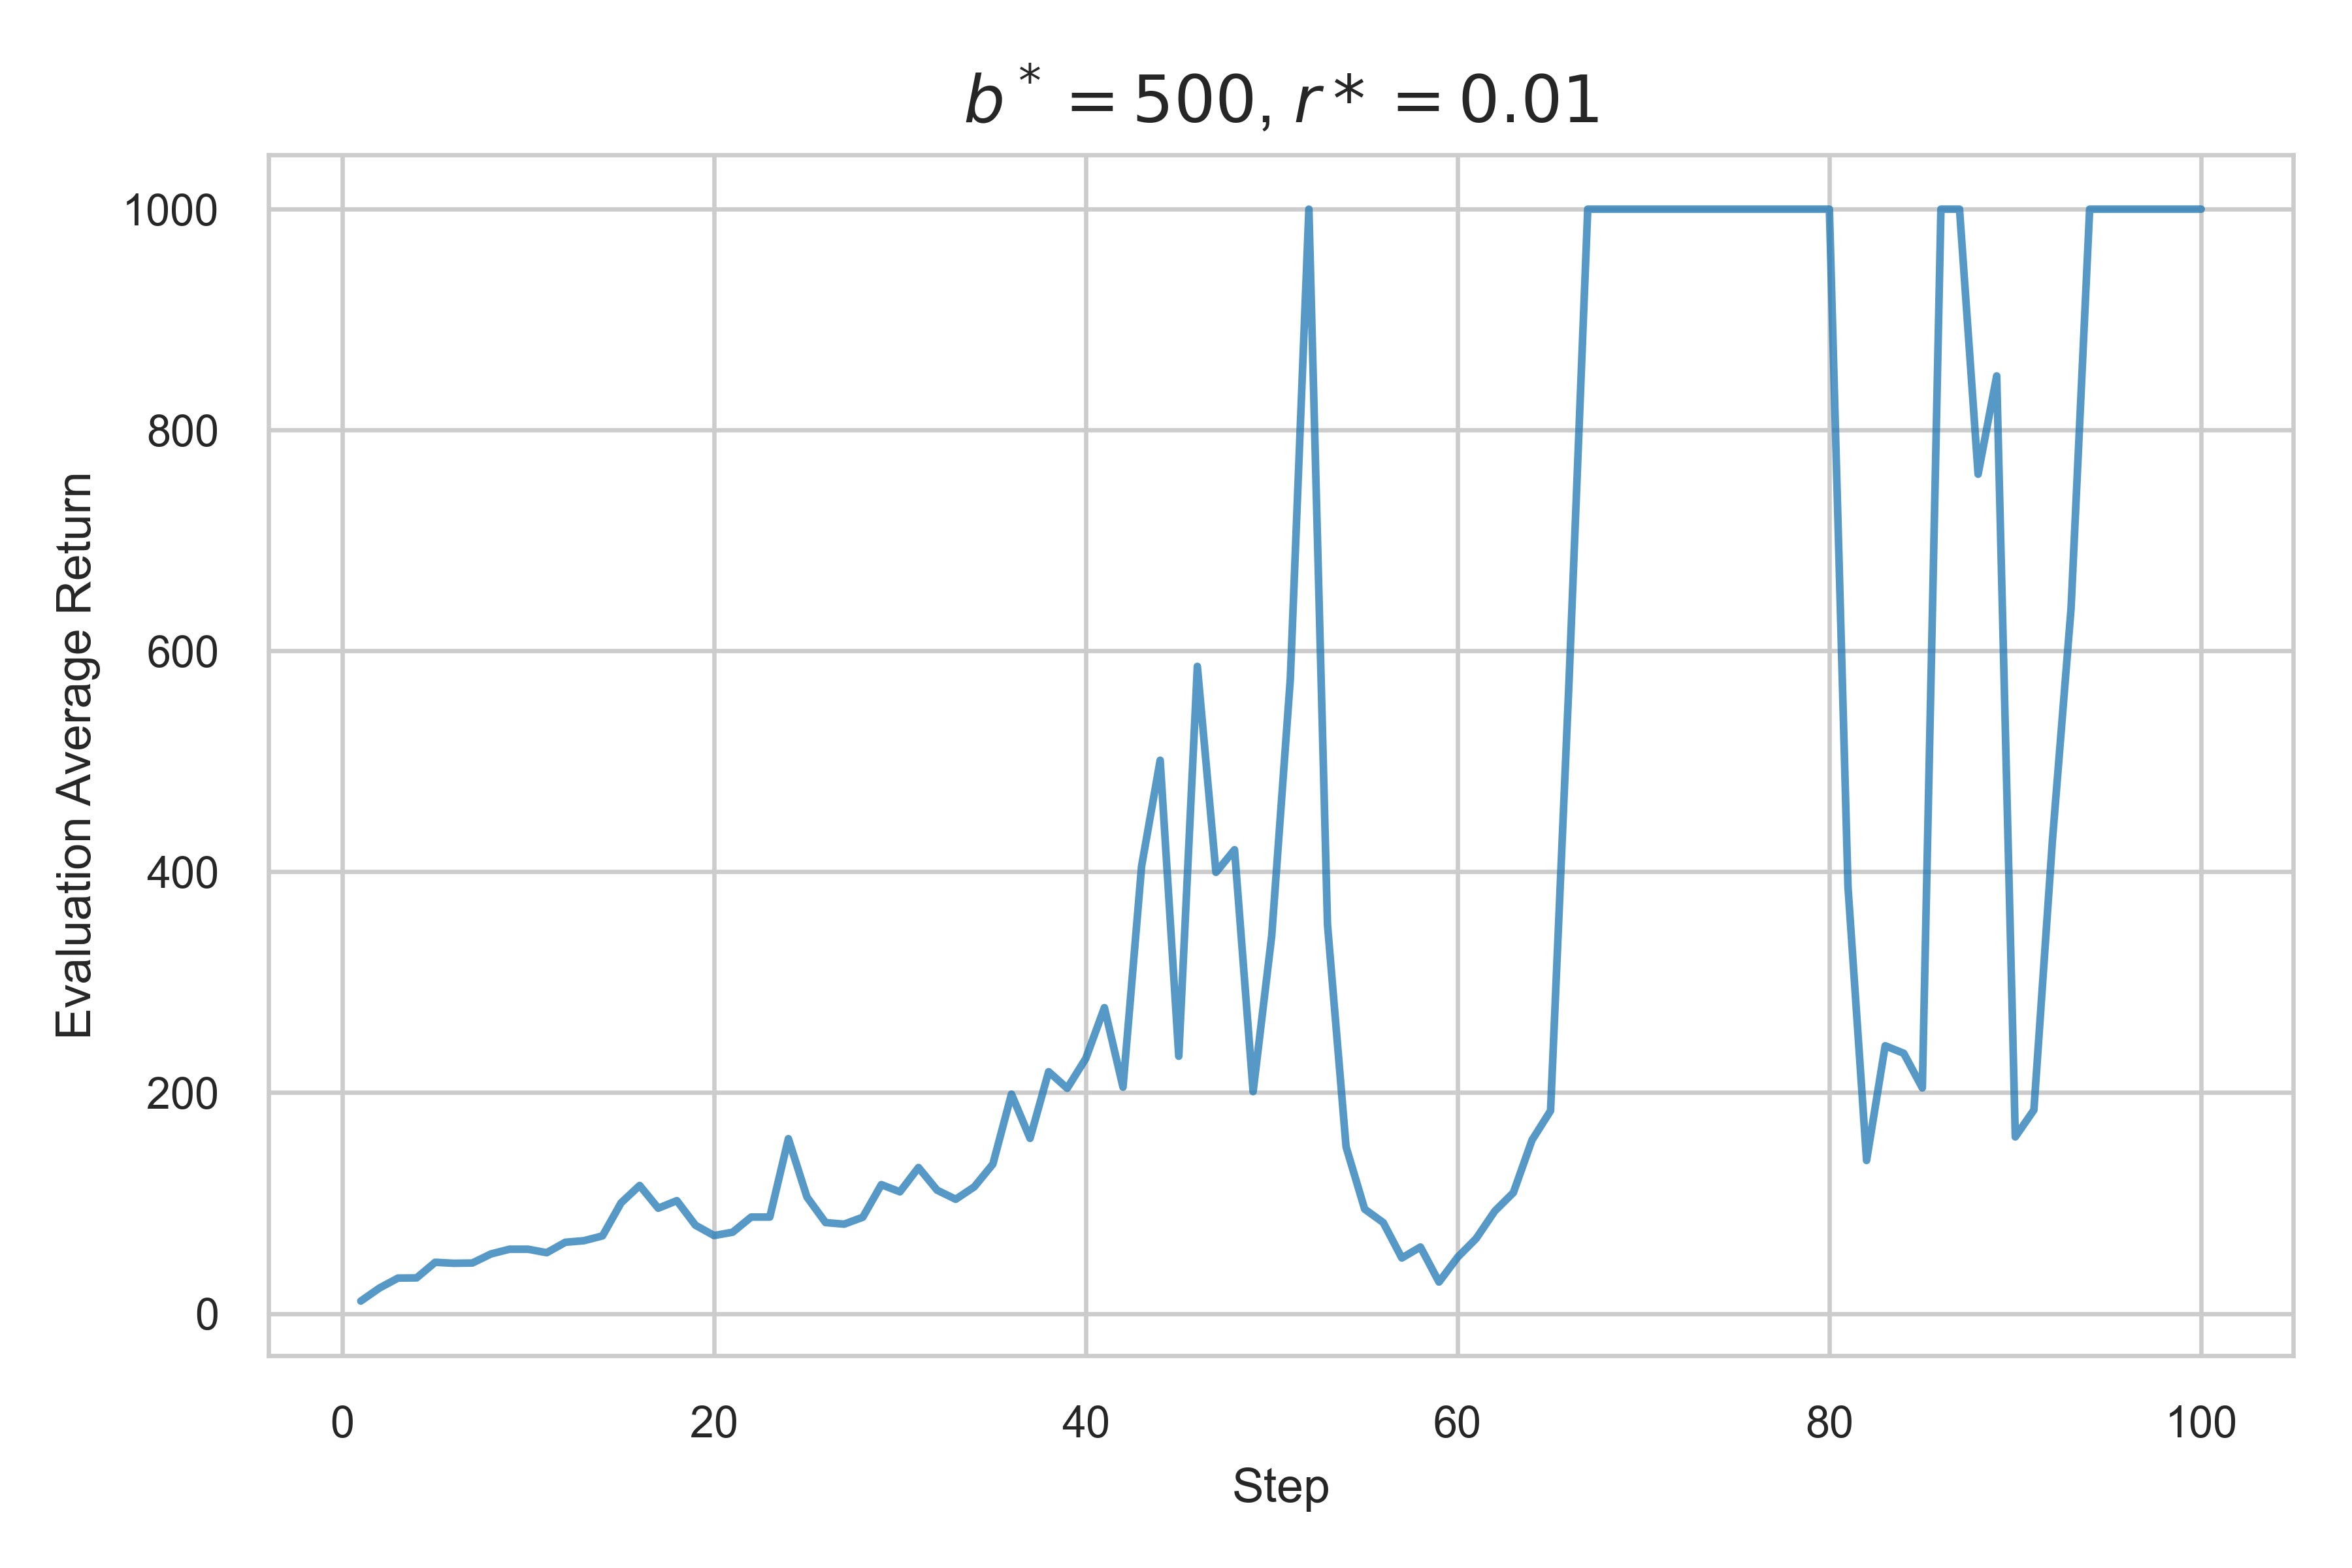
\includegraphics[width=0.6\textwidth]{exp_02.png}
        \caption{Learning curve with optimal settings.}
        \label{fig:2}
    \end{figure}

    \textbf{Command-line Codes}
    \begin{lstlisting}
        echo "Searching for optimal batch and learning rate...";
        for BATCH in 500 1000 2500 5000 7500 
        do
            for LR in 0.005 0.001 0.005 0.01 0.05
            do
                echo "Now running on batch_size=${BATCH}, learning rate=${LR}."
                NAME="q2_b${BATCH}_r${LR}";
                python $1 --env_name InvertedPendulum-v4 --ep_len 1000 --discount 0.9 -n 100 -l 2 -s 64 -b $BATCH -lr $LR -rtg --exp_name $NAME;
            done
        done
    \end{lstlisting}

    \newpage
    \section*{Experiment 3 LunarLander}

    \newpage
    \section*{Experiment 4 HalfCheetah}

    \newpage
    \section*{Experiment 5 HopperV4}

    \textbf{Answers:}

    The averaged evaluation returns with respect to training steps given different $\lambda$ settings is as shown in figure 5. Results show that the evaluation performance at the same timestep increases with a $\lambda$ increasing from 0.00 to 1.00, meaning reducing bias has benefits on the trainig procedure.

    \begin{figure}[thbp]
       \centering
       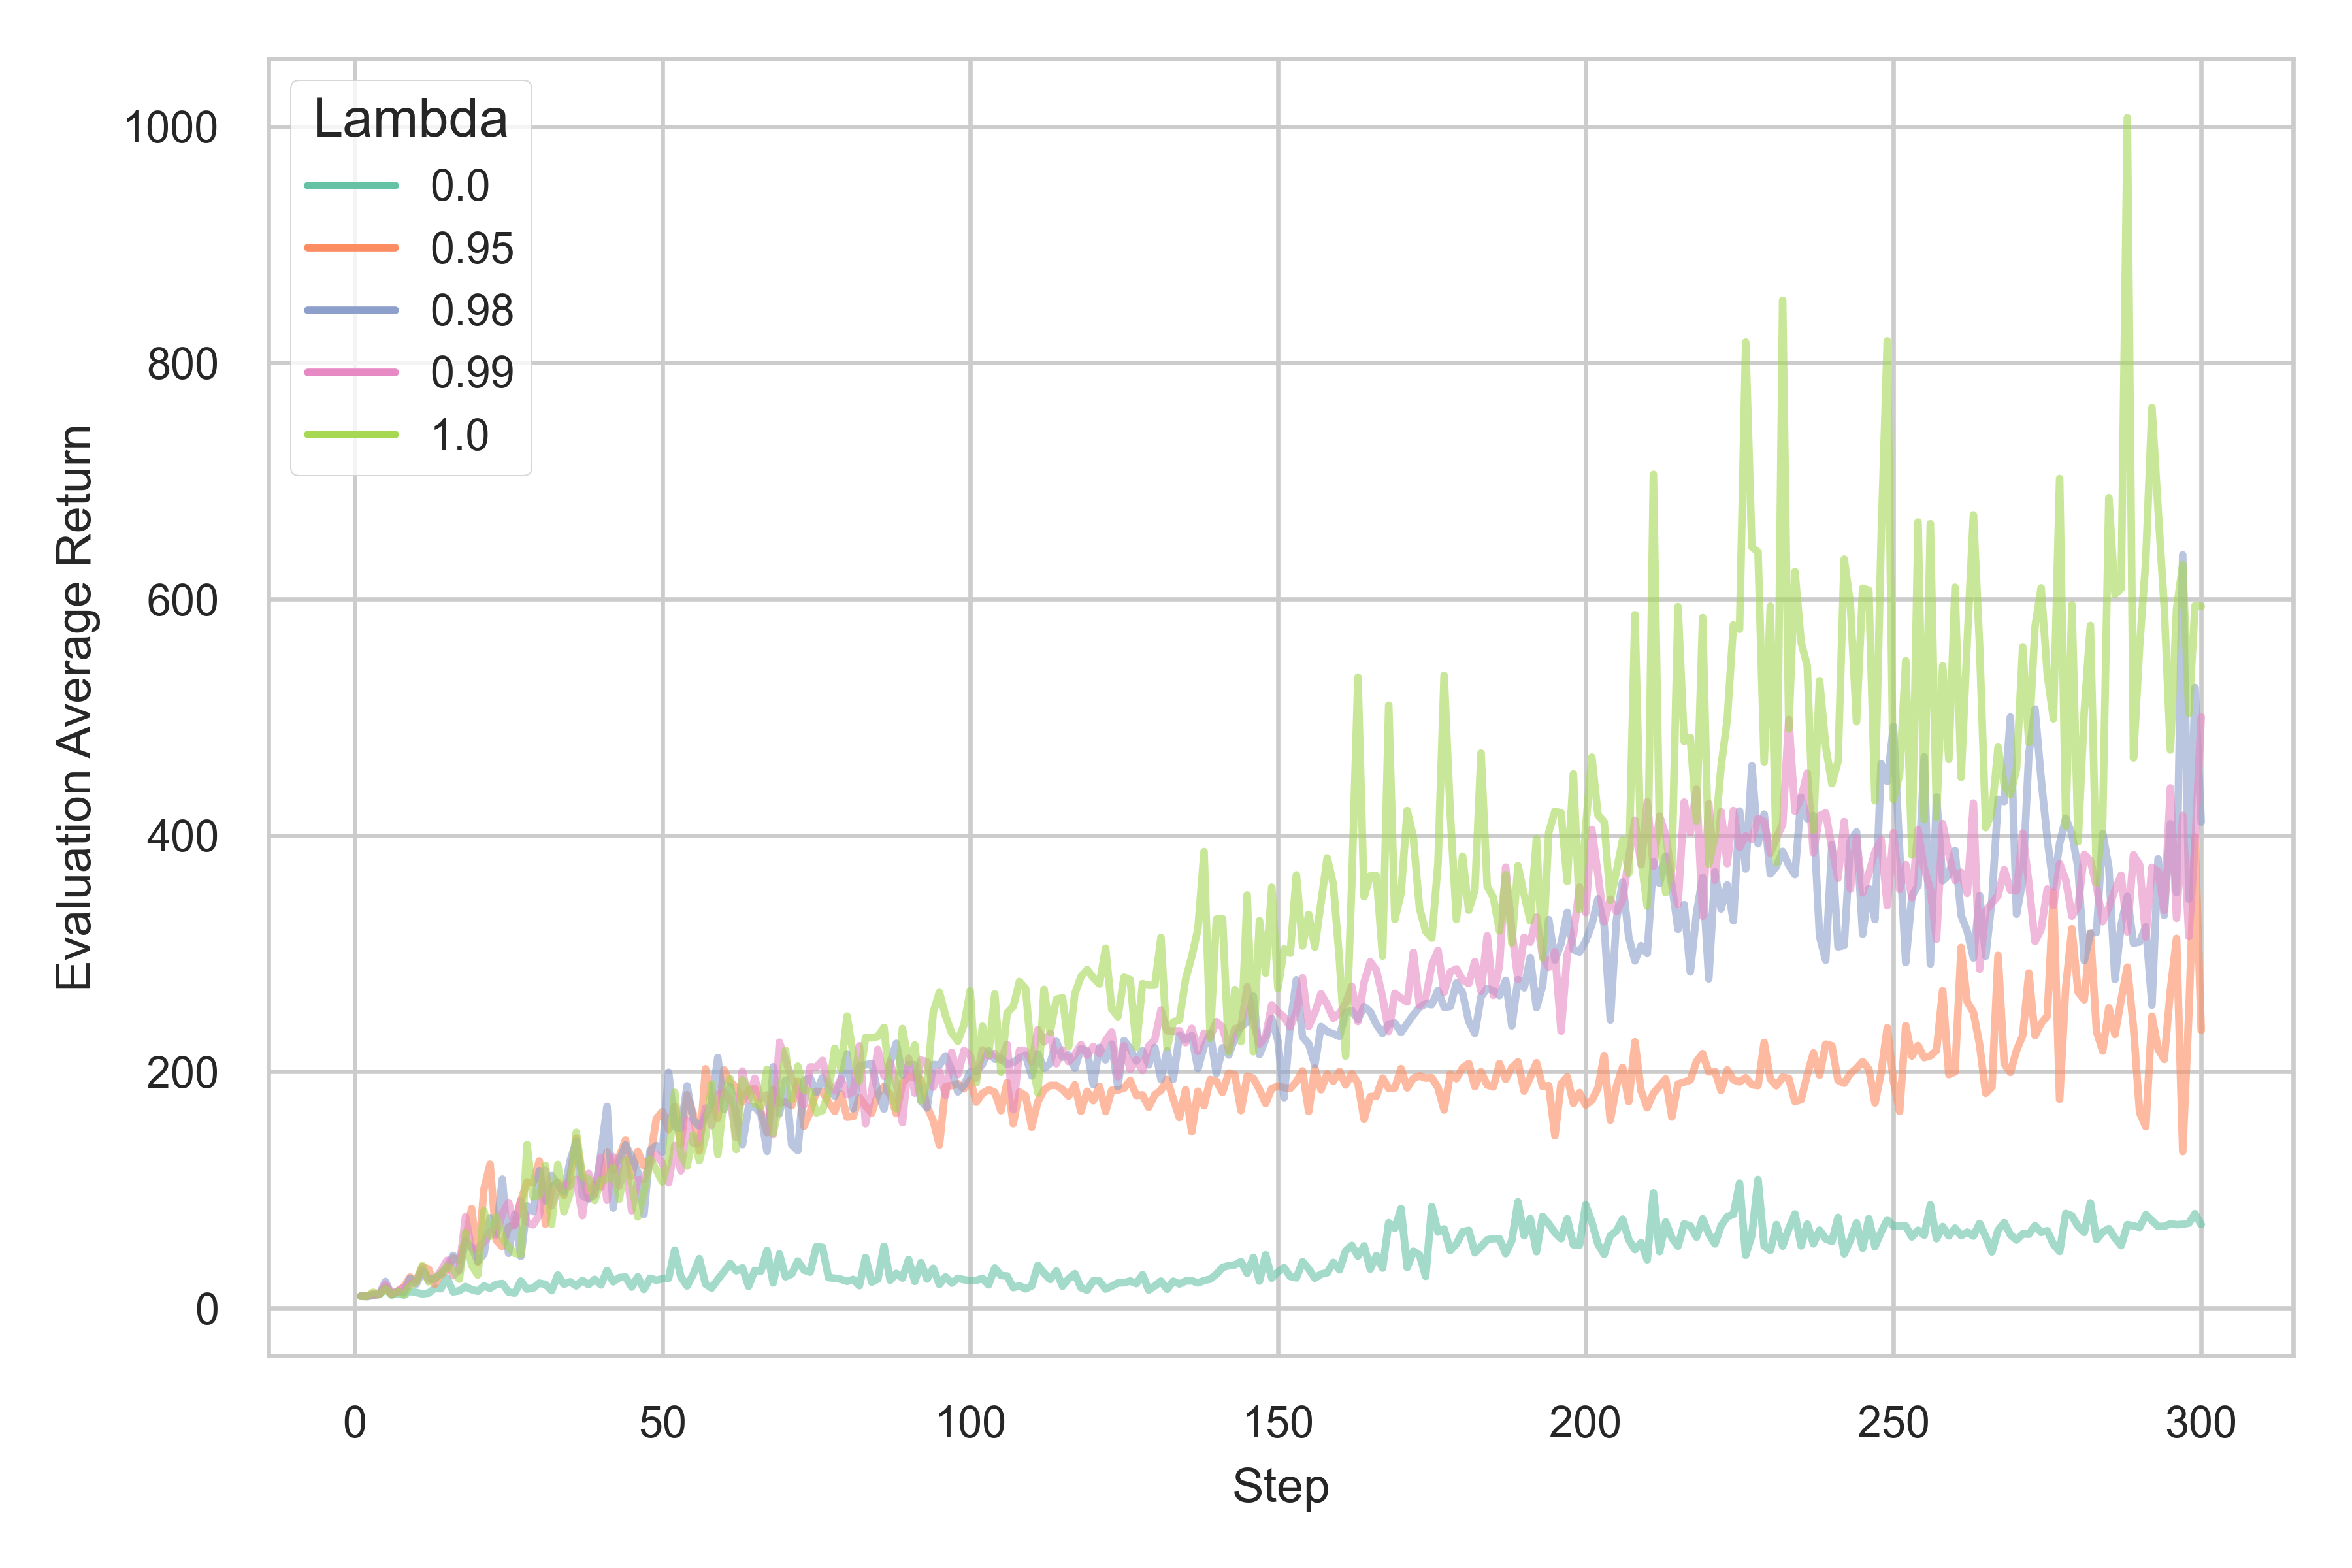
\includegraphics[width=0.9\textwidth]{exp_05.png} 
       \caption{Learning curves for the \texttt{Hopper-v4} with different $\lambda$ settings.}
       \label{fig:5}
    \end{figure}

    \textbf{Command-line Codes}
    \begin{lstlisting}
        echo "Search for the optimal GAE lambda setting...";
        for LAMBDA in 0.00 0.95 0.98 0.99 1.00
        do
            echo "Now running on gae_lambda = ${LAMBDA}.";
            NAME="q5_b2000_r0.001_lambda${LAMBDA}";
            python $1 --env_name Hopper-v4 --ep_len 1000 --discount 0.99 -n 300 -l 2 -s 32 -b 2000 -lr 0.001 --reward_to_go --nn_baseline --action_noise_std 0.5 --gae_lambda $LAMBDA --exp_name $NAME;
        done
    \end{lstlisting}
    
\end{document}